\section{Pulsdetektering}\label{sec_de_im_te_puls}
\textit{I dette afsnit beskrives designet, implementeringen og testen af den valgte pulssensor.}

\subsection{Design} \label{sec_design_puls}
Pulssensoren skal benyttes til at beskrive intensiteten af aktiviteten, som beskrevet i \secref{subsub:ak_int}. Herudfra kan effekten af aktiviteten bestemmes, hvilket vil blive afspejlet som en motiverende faktor i forbindelse med visualisering i GUI. \newline
Pulssensoren SEN-11574 er valgt til dette projekt, da det er en optisk pulssensor og er derfor mere sikker for brugeren, som beskrevet i \secref{sec:pulssensor}. Ydermere er en optisk sensor alsidig i forhold til placering, idet denne type sensor blot kræver en placering over en arterie for at kunne måle pulsen. \newline
Den valgte pulssensor, SEN-11574, kræver en spændingstilkobling på 3~V til 5~V for at være funktionel og forbruger 4~mA ved en forsyning på 5~V. På sensorens board findes et aktivt filter\fxnote{Et aktivt filter er en type af analog elektronisk filter, der anvender aktive bestanddele, såsom en forstærker.} samt en forstærker, som tilsammen øger amplituden for pulsbølgen og normaliserer signalet omkring et referencepunkt, hvilket fjerner DC spænding i signalet. \citep{Murphy2016,Murphy2016_sensor}

Pulssensoren designes således pulsen (BPM) beregnes for brugeren i GAP peripheral og sendes til GAP central, hvilket fremgår af \figref{fig:puls_pseudo}.

\begin{figure}[H]
	\centering
	\includegraphics[scale=0.5]{figures/cDesign/puls_pseudo.png}
	\caption{Illustration af pulssensorens funktioner på GAP peripheral. Pulssensorens algoritme skal registrere tre pulsslag førend pulsen kan bestemmes ud fra disse værdier. Ved tre pulsslag som overskrider tærskelværdien, da vil algoritmen bestemme den gennemsnitlige puls ved brug af disse tre værdier og herefter sende pulsen til GAP central.}
	\label{fig:puls_pseudo}
\end{figure}

Pulssensor opfanger pulssignalet fra brugeren, hvorefter dette signal sendes ind i PSoC 4200M på GAP peripheral. I denne MCU vil algoritmen til beregning af pulsen finde sted, hvilket ses på \figref{fig:puls_pseudo}. \\
Det ønskes at detektere pulsen, ved at beregne varigheden mellem tre pulsslag med udgangspunkt i den systoliske peak, hvilken fremgår af \secref{sec:pulssensor}. Denne peak har større amplitude end peaken for diastole, hvormed det er muligt at foretage signalbehandling således forholdet mellem den systoliske og diastolske peak ændres. Dette vil kunne lade sig gøre, ved at gøre amplituden for den systoliske peak større end peaken for diastole. \\
Denne type signalbehandling vil derfor indebære henholdsvis en division og kvadrering af det oprindelige signal. Dette vil medføre at den største peak i signalet, vil blive forøget i amplitude og de mindre peaks vil opnå en lavere amplitude. Dermed kan en tærskelværdi benyttes til at bestemme antallet af systoliske peaks. \\
Algoritmen designes således, at den kun registrerer et pulsslag når en tidligere sample er over tærskelværdien og den efterfølgende sample er under tærkselværi. Algoritmen benytter yderligere tre pulssalg som overskrider en given tærskelværdi, for derved at kunne bestemme den gennemsnitlige puls med henhold til disse pulsslag. Når algoritmen har registreret tre overskridelser, da vil counteren, som tæller antallet af samples, blive nulstillet. \\
Ved brug af algoritmens counter, vil det gennemsnitlige antal samples som befinder sig mellem tre pulsslag, hvorefter varigheden mellem pulsslagene kan bestemmes med henhold til samplingsfrekvensen i ADCen. Denne samplingsfrekvens konfigureres til 188~Hz, hvilket beskrives i \secref{krav_adc}. Herefter kan algoritmen bestemme pulsen, som de tre pulsslag repræsenterer. Denne puls sendes til GAP central ved brug af bluetooth. 


\subsection{Implementering}
Sensoren har 3 pins til henholdsvis spændingsforsyning, ground og outputsignal. Disse pins kobles til hver sin pin på GAP peripheral. Outputsignalets pin skal designes i programmet PSoC Creator, således MCU'en modtager pulssensorens signale fra den pågældende pin. Dette gøres ved at indsætte henholdsvis en UART serie kommunikationsblok (SCB) og SAR ADC i topdesignet. UART'en bruges for at sensoren og MCU'en kan kommunikere. Standardindstillingerne for denne blok benyttes til konfigurationen af MCUen. \newline
Outputsignalet fra sensoren er et analogt signal, hvormed dette signal skal gennem en ADC, for at skabe en konvertering til et digitalt signal. ADCens design skal derfor konfigurers således denne bearbejder én single ended kanal, inputtet fra pulssensoren. Yderligere indstilles sampleraten for ADcen for den pågældende inputkanal til 35~Hz, jævnfør \secref{krav_adc}. \\
Efter konfigurering af UART og ADC i Topdesignet, skal de korrekte pins indstilles i pinopsætning. UART tildeles interne pins, hvorimod ADC'ens inputpin skal indstilles til den plads, som outputtet fra sensoren er, hvilket i dette tilfælde er pin 2.0. 

Det rå pulssignal vil blive henholdsvis divideret og kvadreret, med henblik på at kunne detektere de systoliske peaks i signalet. Denne signalbehandling fremgår desuden af \figref{fig:behandlet_puls}.

\begin{figure}[H]
	\centering
	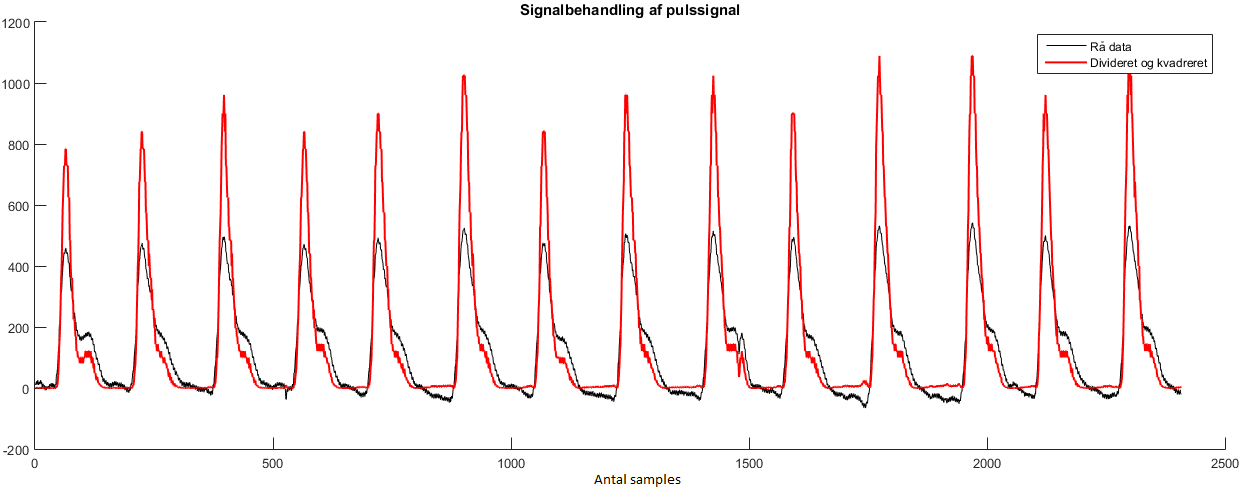
\includegraphics[scale=0.46]{figures/cDesign/puls_ore_behandlet.png}
	\caption{Illustrering af algoritmens signalbehandling (rød kurve), som indebærer en division og kvadrering, af det rå pulssignal (sort kurve).}
	\label{fig:behandlet_puls}
\end{figure}

Det behandlede signals amplitude ses tydeligt forøget, hvorimod de mindre peaks er formindsket. Den store peak i signalet repræsenterer dermed den systoliske periode i hjertecyklussen, hvormed denne peak kan benyttes til at bestemmes BPM for signalet. \\
For at kunne bestemme BPM for signalet, bliver der ydermere implementeret en tærskelværdi. Denne værdi skal signalet overskride for at kunne blive detekteret som et systolisk peak. \\
Tærskelværdien for algoritmen bestemmes med udgangspunkt i en pulsmåling, hvor sensoren er placeret på øreflippen. Denne signaloptagelse fremgår af \figref{fig:taerskel_puls}.

\begin{figure}[H]
	\centering
	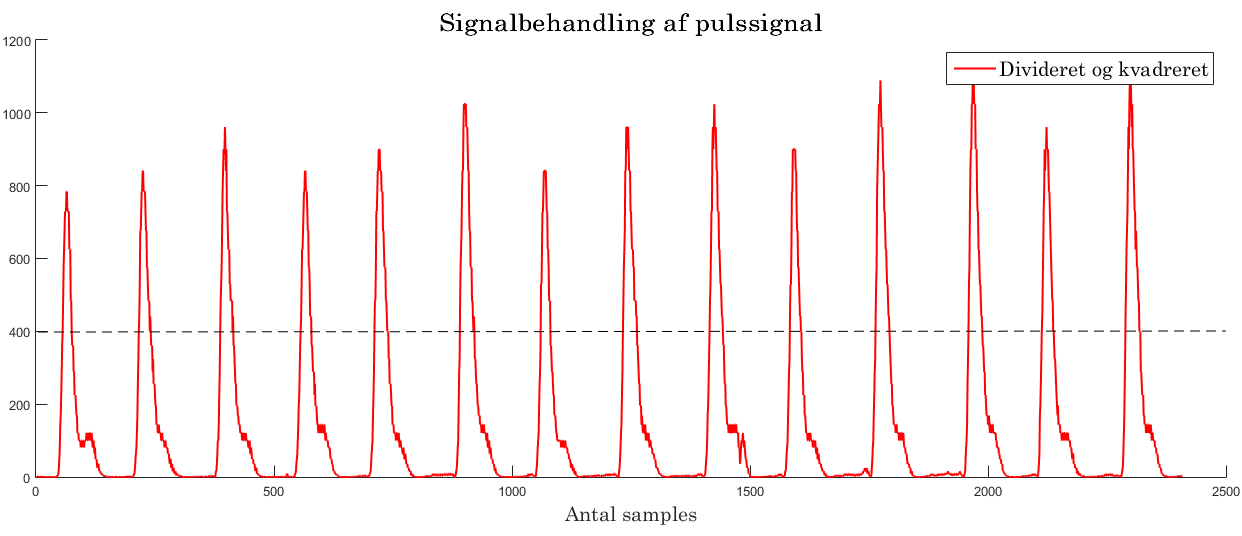
\includegraphics[scale=0.46]{figures/cDesign/puls_taerskel.png}
	\caption{Illustrering af en pulsmåling på en øreflippen (rød kurve), hvortil algoritmens tærskelværdi (sorte, stiplede linje) på 400 er påført.}
	\label{fig:taerskel_puls}
\end{figure}

Den behandlede signal fremgår af figuren, hvortil det er indtegnet en tærskelværdi som alle de systoliske peaks vil kunne overskride.\\
Denne tærskelværdi vil dermed medføre, at det systoliske tryk overstiger tærkselværdien hvortil det diastoliste tryk vil befinde sig under. Algoritmen vil benytte varigheden mellem de forekomne systoliske tryk til at kunne beregne BPM med udgangspunkt i tre peaks. 


\subsection{Test}
Algoritmens funktionalitet testes ved at indsende et simuleret signal, som består af en ensrettet sinusbølge. Dette signal sendes ind i MCUen, hvorefter det undersøges hvorvidt timecounteren detekterer varigheden mellem overskridelser af tærskelværdien. Når pulsen er bestemt, benyttes programmet Real Term til at printe BPM i. \\
Det indsendte signal er en ensrettet sinusbølge som har en frekvens på 0,6~Hz og en samplingsfrekvens på 188~Hz. Ydermere er det array, som indsendes til MCUen, på 1451 samples. Derfor kan det bestemmes hvilken puls, som algoritmen bør printe i Real Term. \\
Der indsendes 1451 samples og der benyttes en samplingsfrekvens på 188~Hz, hvormed arrayet har en længde på 7,7 sekunder. Idet der er tale om en ensrettet sinusbølge på 0,6~Hz, vil der derfor være 9,26 peaks i det indsendte signal. Ydermere vil dette betyde, at algoritmen skal udregne og printe tre værdier for pulsen idet der er cirka 9 peaks. \\
Det fremgår der er 9,26 peaks samt at arrayet har en varighed af 7,7 sekunder, hvormed der er er 0,83 sekunder mellem hver overskridelse af tærskelværdien. Derfor vil det indsendte signal medføre en værdi af 72 BPM. Det er derfor forventeligt, at algoritmen vil beregne og printe en puls som har en værdi af 72 BPM. 

Algoritmen er bestemt til at nulstille sin counter hver gang der er registreret tre overskridelser af tærskelværdien. Derfor vil algoritmen gøre brug af det antal samples som counteren har talt, til at bestemme pulsen for den pågældende periode. \\
Ved at indsende det simulerede signal fremgår det af \figref{fig:timecounter_puls_realterm}, hvordan counteren nulstilles når der er registreret tre overskridelser af tærskelværdien. Ydermere ses det i \tabref{tab:test_puls_realterm}, at Real Term har printer de forventede værdi for BPM.

\begin{figure}[H]
	\centering
	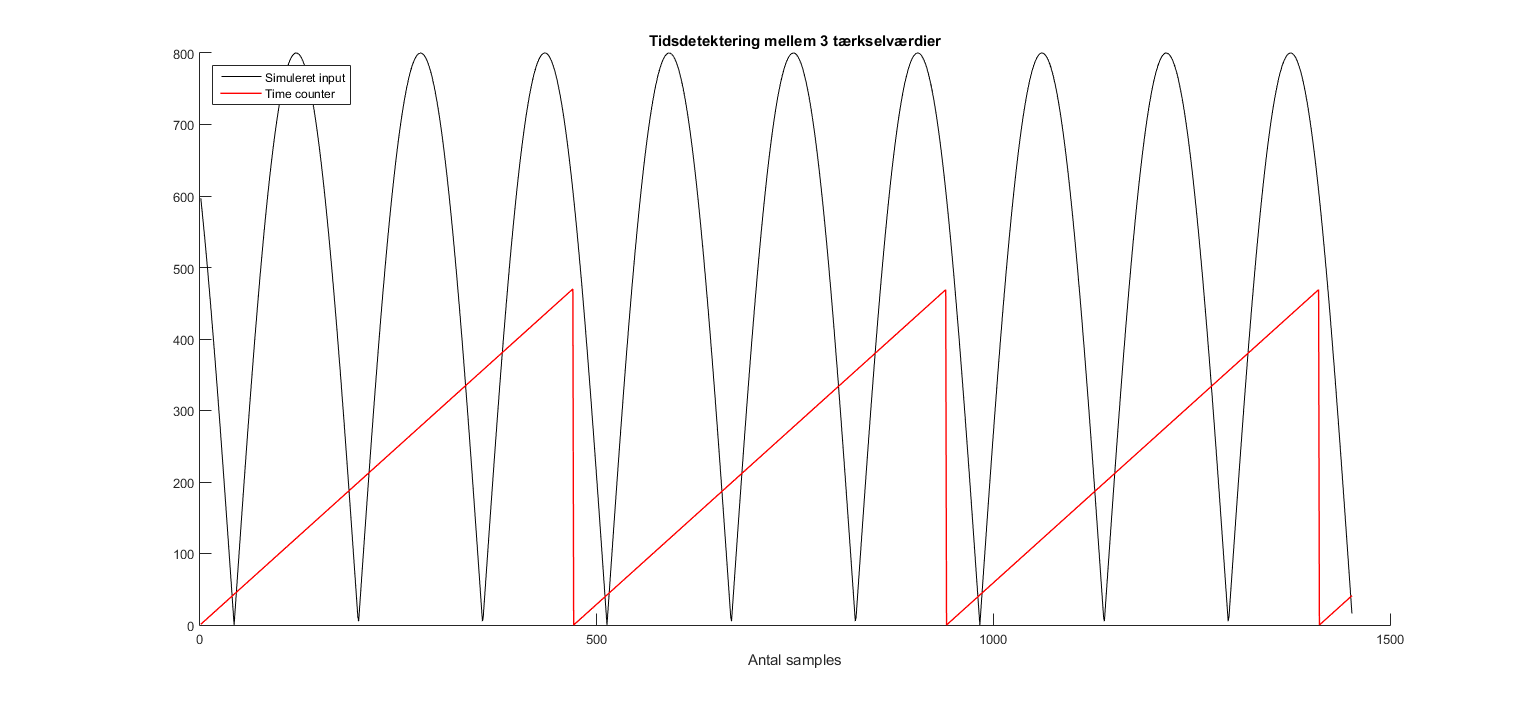
\includegraphics[scale=0.46]{figures/cDesign/timecounter_puls_pic.png}
	\caption{Algoritmens timecounter som tæller op, indtil tre pulsslag har overskredet tærskelværdien, hvorefter timecounter nulstilles og starter samme procedure.}
\label{fig:timecounter_puls_realterm}
\end{figure}

\begin{table}[H]
	\centering
	\begin{tabular}{ccc}
		\hline
		\rowcolor[HTML]{C0C0C0} 
		Forventet værdi [BPM] & Modtaget værdi [BPM] & Afvigelse [\%]\\ \hline
		72 - 72 - 72          & 72 - 72 - 72         & 0\% - 0\% - 0\% \\ \hline
	\end{tabular}
	\caption{I tabellen ses resultaterne fra algoritmens beregning af pulsen på et simuleret inputsignal. Tabellens kolonne; Modtaget værdi, er fra Real Term.}
	\label{tab:test_puls_realterm}
\end{table} \vspace{-0.5cm}

Det fremgår af figuren, at algoritmen tæller counteren op, indtil der er registreret tre overskridelser af tærskelværdien. Herefter beregnes algoritmen pulsen, ud fra det antal samples som counteren har talt. Herefter printes pulsen i Real Term, hvor værdierne er illustreret i tabellen. Det fremgår ydermere, at de modtagede værdier har 0\% afvigelse fra de forventede værdier. \\
Det kan derfor konkluderes, at pulssensoren og den tilhørende algoritme fungerer som tiltænkt ved benyttelse af et simuleret inputsignal. 

Der foretages yderligere to tests, med henblik på at vurdere hvorvidt pulssensoren opfylder de opstillede krav i \secref{puls_krav}. Først testes systemet mens en person er stillesiddende, hvorefter systemet testes ved at løbe på et løbebånd. \\
Først testes pulssensoren og den tilhørende algoritme ved en stillesiddende aktivitet. Dette udføres ved at påføre sensoren på en forsøgsperson, hvorefter denne person løber med en konstant hastighed på et løbebånd. Yderligere vil der blive benyttet en pulsmåler i form af ......., som benyttes som reference for den beregne puls af algoritmen. 







